\chapter{Conclusion}\label{chap:conclusion}

  \begin{figure}
    \centering
    \begin{minipage}{10cm}
      \centering
      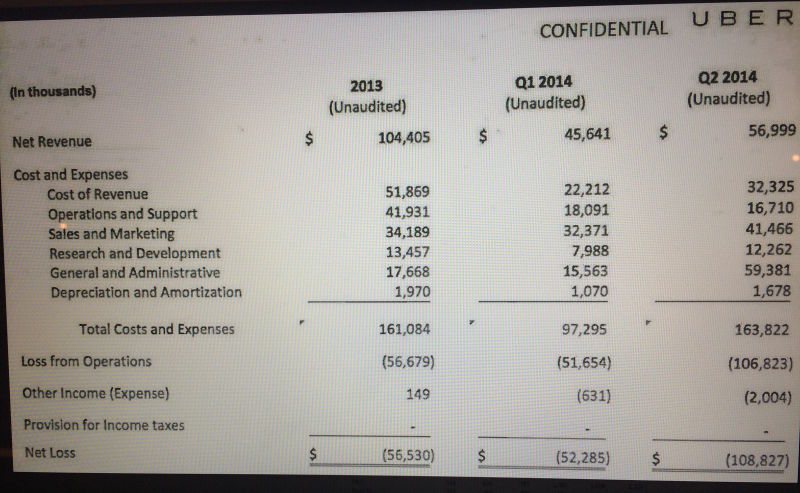
\includegraphics[width=10cm]{inc/uber_net_revenue.png}
      \caption[Uber's Net Revenue]{Uber's Net Revenue~\parencite{uber2015}}
      \label{fig:uber_net_revenue}
    \end{minipage}
  \end{figure}

  Uber has yet to turn a profit (Figure~\ref{fig:uber_net_revenue}; Figure~\ref{fig:uber_profit_loss}; Figure~\ref{fig:uber_cash_flow}). According to~\cite{newcomer2015}, the company is generating \$470M in operating losses on \$415M in revenue. In addition, the company appears to be spending aggressively in China, as it experiments with the UberPool service. Note that this is prior to the company subtracting any internal costs, such as R\&D. As humans are currently taking home 80\% of the revenue from daily transactions, we recommend that Uber continue their shift towards autonomous cars -- as over time (cf.\ Figure~\ref{fig:autonomous_vehicles}), they will see an increase in overall profitability.

  \begin{figure}
    \centering
    \begin{minipage}{10cm}
      \centering
      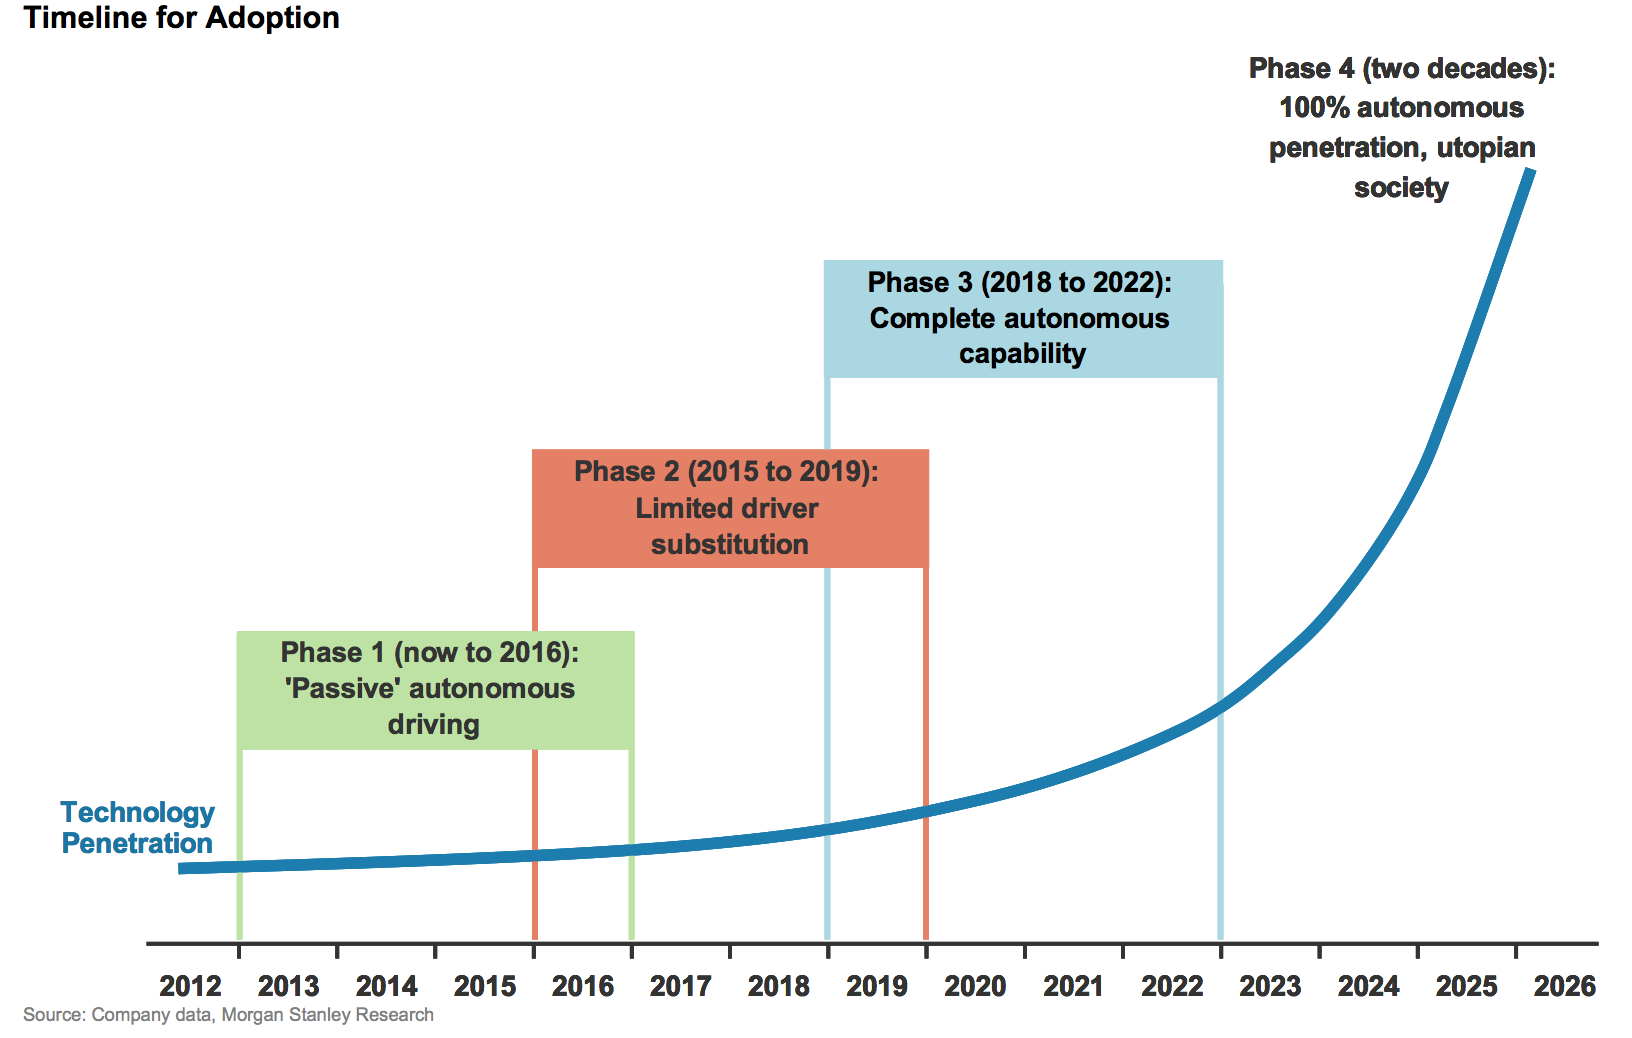
\includegraphics[width=10cm]{inc/autonomous_vehicles.png}
      \caption[Timeline for the Adoption of Autonomous Vehicles]{Timeline for the Adoption of Autonomous Vehicles~\parencite{owyang2015}}
      \label{fig:autonomous_vehicles}
    \end{minipage}
  \end{figure}
